\section{Hardware Design} \label{sec:design}

Our main design goal is to improve the throughput of the lattice-based key encapsulation scheme FrodoKEM \cite{frodokem} when implemented in hardware. As described in Section \ref{sec:related}, FrodoKEM is one of the leading conservative candidates submitted to the NIST post-quantum standardisation effort \cite{nistpq}, currently a semi-finalist in the process. Moreover, it has been shown to have appealing qualities which make it an ideal candidate for hardware implementations; such as having a power-of-two modulus and significantly easier parameter selection. However, a complete exploration of the possible hardware optimizations applicable to FrodoKEM has yet to be done. For instance, previous implementations do not consider parallelisations or other design alternatives capable of significantly improving the throughput.

As described in Section \ref{sec:related}, FrodoKEM requires heavy use of PRNG / seed expanding. In the algorithm specifications, it is suggested to use either SHAKE or AES. In particular, the most computationally intensive operations, such as Line \ref{alg:lwe} of Algorithm \ref{alg:decaps}, require 410k or 953k 16-bit pseudo-random values, depending on the parameter set used. In order for PRNG not to be the bottle-neck it needs to achieve a very high throughput (ideally with relatively low area consumption) typically in the range of 16 bits per clock cycle. In a previous hardware design, proposed by Howe et al. \cite{howe2018standard}, high throughput for the PRNG was achieved by pre-calculating randomness and storing it in BRAM. Random data newly calculated was then written into the memory, overwriting the random data previously stored. This is an efficient approach, however a more efficient PRNG that would not require BRAM usage, potentially increasing the operating frequency of the design, and thus improve its throughput. Moreover, parallelisations was not possible for this design, as this would require a faster SHAKE design, increasing the area consumption by 3-8x \cite{bertoni2012keccak}. The area consumption of SHAKE (or AES) was an issue with the previous design. For example, cSHAKE used within FrodoKEM-640 Encaps occupies 42\% of the overall hardware resources~\cite{howe2018standard}. 

To improve the parallelism of our implementation, we further the discussions in Section \ref{sec:shake}. That is, we further the investigations that research PRNG alternatives in post-quantum cryptographic schemes and translate this into hardware. As with other design explorations, this means we do not completely comply with the specifications (and test vectors) by not using a NIST standard. However, their security arguments that AES is an `ideal cipher' for use as an seed expander still apply as we replace this with Trivium, as it has analogous security properties of being indistinguishable from random. Moreover, with NIST's lightweight competition happening in parallel, it is likely that there will be future NIST standards that are more efficient than SHAKE. We may also see specific use-cases where an alternative PRNG is preferred to SHAKE. Thus, considering alternative PRNGs as a design exploration is an important contribution to the standardisation process.

We explored several options and we decided to integrate into our design an unrolled x32 Trivium \cite{de2008trivium} module. This is compatible with the security requirements of the FrodoKEM submission. In fact, the authors of the algorithm suggest that replacing the PRNG with another, that still has good statistical pseudo-random properties, still guarantees the security claims of FrodoKEM. The Trivium architecture we integrate has high throughput and maintains the cryptographic security required in the FrodoKEM specifications, thus perfectly fits our needs. %The primary reason the proposed designs have achieved both high throughput and practical area consumption is through this idea of replacing the PRNG.

\vspace{-0.2cm}

\subsection{Hardware Optimisations}

In order to fully explore the potential of FrodoKEM in hardware, we propose several architectures characterized by different design goals (in terms of throughput). We use the proposed architecture to implement key generation, encapsulation, and decapsulation, on two sets of parameters proposed in the specifications: FrodoKEM-640 and FrodoKEM-976. Our designs use 1x, 4x, 8x, and 16x parallel multiplications during the most computationally intensive parts in FrodoKEM. These operations are the LWE matrix multiplications of the form:
%The following is the LWE calculation of the type: 
\begin{equation}
\mathbf{B} = \mathbf{S} \mathbf{A} + \mathbf{E}, \label{lwe}
\end{equation}
 required in key generation, encapsulation, and decapsulation. In the previous hardware implementations of FrodoKEM, the operations of the type of Equation \ref{lwe} took approximately 97.5\% of the overall run-time of the designs \cite{howe2018standard}. As in the literature, we exploit DSP slices on the FPGA for the multiply-and-accumulate (MAC) operations required for matrix multiplication. Hence, each parallel multiplication of the proposed designs requires its own DSP slice. The LWE matrix multiplication component incurs a large computational overhead. Because of this, it is an ideal target for optimizations, and for our optimizations we heavily rely on parallelisations. Firstly we describe the basic LWE multiplier, that includes just one multiplication component. Then we describe how this core is parallelised, allowing us to significantly improve the throughput.
 
\begin{figure}[htbp]\centering
    %\advance\leftskip-1cm
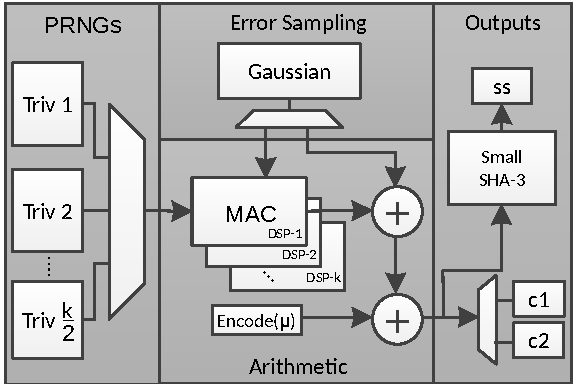
\includegraphics[scale=0.75]{figures/arch_new.pdf}
\caption{A high-level overview of the proposed hardware designs for FrodoKEM for $k$ parallel multipliers. The architecture is split into sections `PRNGs' for Trivium modules, `Error Sampling' for the Gaussian sampler, `Arithmetic' for the LWE multiplier, and `Outputs' for the shared-secret and ciphertexts.}\label{arch}
\end{figure}

Figure \ref{arch} shows a high-level overview of the hardware architecture and the following descriptions will link to the design overview. The \texttt{Arithmetic} part of the LWE core is essentially made by vector-matrix multiplication (that is, $\mathbf{S}[\text{row}]\times \mathbf{A}$), addition of a \texttt{Gaussian} error value (that is, $\mathbf{E}[\text{row},\text{col}]$), and, when needed, an addition of the \texttt{Encoding} of message data. Since the matrix $\mathbf{S}$ consists of a large number of column entries (either 640 or 976) but only 8 row entries (for both parameter sets), we decided to implement a vector-matrix multiplier, instead of (a larger) matrix-matrix one. By doing this, we can reuse the same hardware architecture for each row of $\mathbf{S}$, saving significant hardware resources. Each run of the row-column MAC operation exploits a DSP slice on the FPGA, which fits within the 48-bit MAC size of the FPGA. The DSP slice is ideal for these operations, but it also ensures constant computational run-time, since each multiplication requires one clock cycle. Once each row-column MAC operation is completed, an error value is added from the CDT sampler. These outputted ciphertext values are also consistently added into an instantiation of SHAKE, which is required to calculate the shared secret. This process is pipe-lined to ensure high throughput and constant run-time. 

%cSHAKE is still required for RO, this can be done in parallel to the next KEM calculation.

To avoid using BRAM (for pre-computing some of the matrix $\mathbf{A}$) and while keeping the throughput needed by the MAC operations of the matrix multiplications, the designs require 16 bits of pseudo-randomness per multiplication per clock cycle. Thus, for every two parallel multiplications we require one Trivium instantiation, whose 32-bit output per clock cycle is split up to form two 16-bit pseudo-random integers. This is shown in \texttt{PRNGs} part of Figure \ref{arch}. This pseudo-randomness forms the matrix $\mathbf{A}$ in Equation \ref{lwe}, whereas the matrix $\mathbf{S}$ and $\mathbf{E}$ require randomness taken from \texttt{Gaussian} sampler. The cumulative distribution table (CDT) sampler technique has been shown to be the most suitable one for hardware \cite{howe2018practical} and thus we use it in our designs. However, compared with previous works, we replace the use of AES as a pseudo-random input with Trivium. This ensures the same high throughput, but requires significantly less area on the FPGA.

\begin{figure}[htbp]\centering
    %\advance\leftskip-1cm
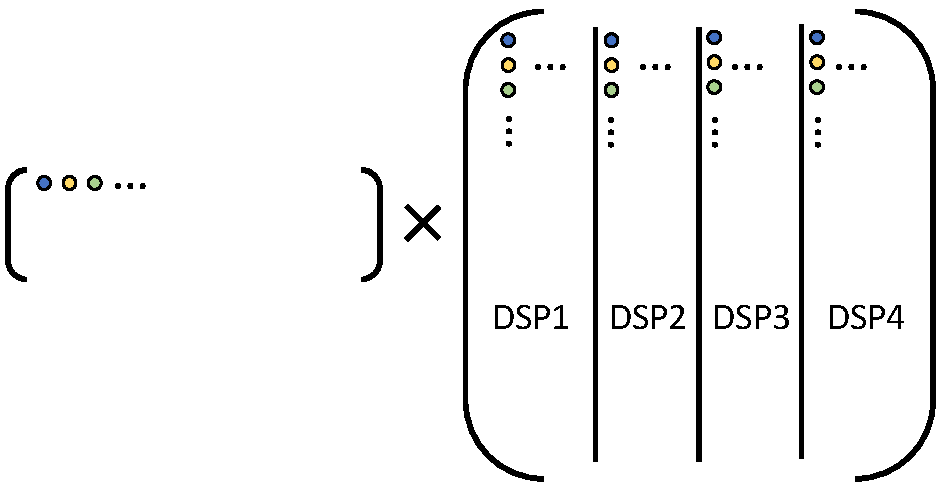
\includegraphics[scale=0.45]{figures/parallel.pdf}
\caption{Parallelising matrix multiplication, for $\mathbf{S}\times\mathbf{A}$, used within LWE computations for an example of $k=4$ parallel multiplications, using $k=4$ DSPs on the FPGA.}\vspace{-0.35cm}
\label{parallel}
\end{figure}

The technique we use to parallelise Equation \ref{lwe} is to vertically partition the matrix $\mathbf{A}$ into $k$ equal sections, where $k$ is the number of parallel multiplications, and DSPs, used. This is shown in Figure \ref{parallel} for $k=4$ parallel multiplications, utilizing 4 DSP slices for MAC. Each vector on the LHS of Figure \ref{parallel} remains the same for each of the $k$ operations. We repeat this vector-matrix operation for the $\bar{n}=8$ rows of the matrix $\mathbf{S}$. This technique is used across all designs for the three cryptographic modules to ensure consistency.  

In order to produce enough randomness for these multiplications to have no delays, we need one instance of our PRNG, Trivium, for every two parallel multiplications. This because each element of the matrix $\mathbf{A}$ is set to be a 16-bit integer and each output from Trivium is 32 bits, that is, two 16-bit integers. As the Trivium modules are relatively small in area consumption on the FPGA (169 slices), an increase in $k$ is fairly scalable as an impact on the overall design.

\vspace{-0.2cm}

\subsection{Efficient First-Order Masking}

We implement first-order masking scheme (discussed in Section \ref{sec:mask}) to the decapsulation operation $\mathbf{M} = \mathbf{C} - \mathbf{B}'\mathbf{S}$, as this is the only instance where secret-key information is used. Our design allows us to implement this masking schema without affecting the area consumption or throughput. This is achieved by using the optimizations previously discussed. The matrix $\mathbf{S}$ is split using the same technique from Figure \ref{parallel} and our secret shares are generated by using the Trivium modules as a PRNG source. By computing these calculations in parallel, the masked calculation of $\mathbf{M}$ has the same run-time as the one needed to complete the calculation when masking is not used. We ensure that the same row-column operation during the matrix multiplication is not computed in each parallel operation, to circumvent any attack that might combine the power traces and essentially remove the masking.